\documentclass[11pt]{article}
\usepackage{geometry}
 \geometry{
 a4paper,
 total={170mm,257mm},
 left=20mm,
 top=20mm,
 }
\usepackage{xspace}
\usepackage{tcolorbox}
\tcbuselibrary{listings}
\newtcblisting{code}{
  listing only,
  nobeforeafter,
  after={\xspace},
  hbox,
  tcbox raise base,
  fontupper=\ttfamily,
  colback=lightgray,
  colframe=lightgray,
  size=fbox
  }
\usepackage{tikz}
\usetikzlibrary{shapes.geometric, arrows}
\usetikzlibrary{matrix}
\author{Gerrit R}
\title{Sudoku Solver Technical Specifications}
\date{2024}

\begin{document}
\maketitle
\section{Introduction}
This project takes an input file containing an 
(unsolved) sudoku board in the form of a CSV, and solve it, using Rust. This document is made with \LaTeX.

\section{Wave Function Collapse}
Wave function collapse is an algorithm that has a scary name, but 
is surprisingly simple, if resource intensive. The idea is that if 
an item has an unknown state (like a sudoku tile that isn't filled in), 
conceptually it can be considered in all of the states it could possibly be in.
For exmpale, given a very simple psudo-sudoku board, only going up to 4 (as opposed to 9):\\
\begin{center}
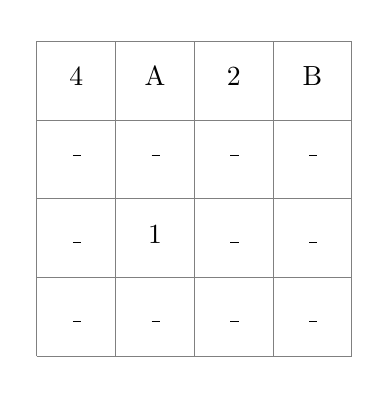
\begin{tikzpicture}
\draw[step=0.5cm,color=gray,xscale=2,yscale=2] (-1,-1) grid (1,1);
\matrix[matrix of nodes,nodes={inner sep=0pt,text width=1cm,align=center,minimum height=1cm}]{
4 & A & 2 & B \\
\_ & \_ & \_ & \_ \\
\_ & 1 & \_ & \_ \\
\_ & \_ & \_ & \_\\};
\end{tikzpicture}
\end{center}
Consider A and B to be tiles that aren't filled in. If only the top row is considered, the wave
function collapse algorithm would say that both $A$ and $B$ are in both a state of being 1 
and a state of being 3, at the same time! But if the program then considers tiles outside the top row,
it sees that in the second column, which $A$ belongs to, there is a 1. Since $A$ now cannot be $\{1, 3\}$, 
instead the set of all its current possible states is $\{3\}$. Because of this, it's real state is known, and it 
"collapses" into a single state, namely being 3. Since $A$ is now 3, the set of all of $B$'s states is now simply
$\{1\}$, meaning it too can collapse into a single state. \\
Note that this method does have limitations. There is a point where the function breaks down. For example, given this simple board:
\begin{center}
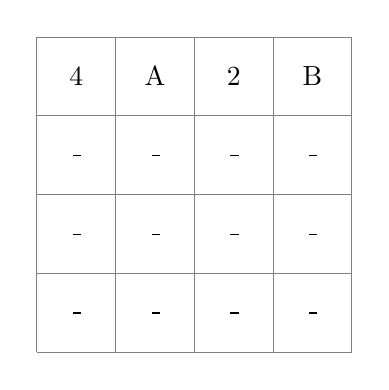
\begin{tikzpicture}
\draw[step=0.5cm,color=gray,xscale=2,yscale=2] (-1,-1) grid (1,1);
\matrix[matrix of nodes,nodes={inner sep=0pt,text width=1cm,align=center,minimum height=1cm}]{
4 & A & 2 & B \\
\_ & \_ & \_ & \_ \\
\_ & \_ & \_ & \_ \\
\_ & \_ & \_ & \_\\};
\end{tikzpicture}
\end{center}
In this circumstance there is no way for the algorithm to know the exact state of $A$ or $B$, and thus will require human intervention.
\section{Large picture process}
\begin{center}
\tikzstyle{startstop} = [rectangle, rounded corners, minimum width=3cm, minimum height=1cm,text centered, draw=black, fill=red!30]
\tikzstyle{io} = [trapezium, trapezium left angle=70, trapezium right angle=110, minimum width=3cm, minimum height=1cm, text centered, draw=black, fill=blue!30]
\tikzstyle{process} = [rectangle, minimum width=3cm, minimum height=1cm, text centered, draw=black, fill=orange!30]
\tikzstyle{decision} = [diamond, minimum width=3cm, minimum height=1cm, text centered, draw=black, fill=green!30]
\tikzstyle{arrow} = [thick,->,>=stealth]

\begin{tikzpicture}[node distance=1.75cm]
  \node (start) [startstop] {Command line perameters};
  \node (pro1) [process, below of=start] {Seek input file};
  \node (dec1) [decision, below of=pro1, yshift=-0.6cm] {Is is usable?};
  \node (stop) [startstop, right of=dec1, xshift=3cm] {Stop, provide error message};
  \node (pro2) [process, below of=dec1, yshift=-0.6cm] {Format input into data structure};
  \node (wfc) [io, below of=pro2] {Wave Function Collapse};
  \node (dec2) [decision, below of=wfc, yshift=-1.5cm] {Is the puzzle solvable?};
  \node (error) [startstop, right of=dec2, xshift=3.6cm] {Stop, provide error message};
  \node (out) [startstop, below of=dec2, yshift=-1.5cm] {Output solved sudoku};

  \draw [arrow] (start) -- (pro1);
  \draw [arrow] (pro1) -- (dec1);
  \draw [arrow] (dec1) -- node[anchor=south] {no} (stop);
  \draw [arrow] (dec1) -- node[anchor=east] {yes} (pro2);
  \draw [arrow] (pro2) -- (wfc);
  \draw [arrow] (wfc) -- (dec2);
  \draw [arrow] (dec2) -- node[anchor=south] {no} (error);
  \draw [arrow] (dec2) -- node[anchor=east] {yes} (out);
\end{tikzpicture}
\end{center}
\section{Why Rust/How Rust?}
The Rust language is ideal for this project for many reasons. Primarily, the type system it offers, combined with the
pattern matching it provides, allows for excellent error handling for avoiding issues at runtime. Secondly, similar to the C family,
Rust is a relatively fast language, which is imperative for this project, due to the nature of the algorithm in use. \\
Because of the Rust compiler and the Rust Foundation's clear stance on what idiomatic Rust looks like, using the common naming conventions shouldn't be an issue.
For example, variables in snake\_case, UpperCamelCase for data structures, SCREAMING\_SNAKE\_CASE for statics, etc. If something isn't idiomatically named, the 
Rust compiler will throw a warning. As with most Rust projects, defining what pardigm is in use is difficult, as Rust provides optionality for everything 
from (something like) OOP to (something like) functional programming. This project uses mainly a OOP design pattern, basing around data 
structures and associated methods, however tends slightly into a functional paradigm when dealing with immutable/mutable references.
Discussing the use of specific crates, command line input is managed by the Clap crate and I/O is managed by the CSV crate, although the serde create is utilized for
deserialization of the config.json file.

\section{Errors}
Rust does its very best not to error, and -slightly less then- its best not to panic. To achieve this, any time a operation might not complete its 
operation it returns the Result enum, in the form of either Ok() or Err(). This is dandy for an aspiring programmer, however different Rust creates (or even sub sections inside
the standard library) return different, non-uniform types inside the Err(). To avoid issues with unknown types, whenever an error needs to be returned, it should be transformed into the Error struct
provided in error.rs. 

\section{File Formatting}
As of this moment, the executable does not care if the tiles are in order. That being said, it does have some specifications to properly load in a CSV. Firstly, actually using a CSV.
CSV stands for Comma Seperated Value, where each cell in the spreadsheet (CSVs can be thought of as a spreadsheet's file format, like bitmap for an image) is represented by a value followed by a comma:\\
\begin{center}
  1, 1, 1, 1, 1, 1, 1, 1, 1\\
  2, 2, 2, 2, 2, 2, 2, 2, 2\\
  3, 3, 3, 3, 3, 3, 3, 3, 3\\
  4, 4, 4, 4, 4, 4, 4, 4, 4\\
  5, 5, 5, 5, 5, 5, 5, 5, 5\\
  6, 6, 6, 6, 6, 6, 6, 6, 6\\
  7, 7, 7, 7, 7, 7, 7, 7, 7\\
  8, 8, 8, 8, 8, 8, 8, 8, 8\\
  9, 9, 9, 9, 9, 9, 9, 9, 9\\
\end{center}
Note that this table is 9 rows long, and is 9 columns wide, this is the format that will be loaded properly, as it is the format of a sudoku board. However, also note that this board has 
abundent white space, and will not be loaded properly and is formatted this way for visability. This board (with whitespace trimmed) would go directly into memory in this format, however if the board has holes, like so:\\
\begin{center}
  1, 1, 1, 1, 1, 1, 1, 1, 1\\
  2, 2, 2, 2, 2, 2, 2, 2, 2\\
  3, 3, 3,  , 3, 3, 3, 3, 3\\
  4, 4, 4, 4, 4, 4, 4, 4, 4\\
  5, 5, 5, 5, 5, 5, 5, 5, 5\\
  6, 6, 6, 6, 6, 6, 6, 6, 6\\
  7, 7, 7, 7, 7, 7, 7, 7, 7\\
  8, 8, 8, 8, 8, 8, 8, 8, 8\\
  9, 9, 9, 9, 9, 9, 9, 9, 9\\
\end{center}
Notice that the board has a hole in the 4th column 3rd row, and due to this it will be loaded as a Vec$<>$ of it's possabilities. If the -a flag is set, then 
during the loading process the program will try to load the first number it can find, assuming it's within the board. Some CSVs can have a header row, a row at the start that might 
be used, well, as a header for whatever spreadsheet it was exported from. If this is the case, the -h flag will acount for it. 

\section{Config}
The provided config file is a proof of concept. Without overriding, the executable looks for $\sim$/.config/sudoku-solve/config.json, and will attempt to load it. As of now, it only
provides a default for the name of the output file, but is easily extensible.

\section{Running, Tests}
This project is run the same as any other Rust projects, using "cargo run". That being said, it does have one required argument: the path of a file, to load as a CSV.
It also has a few optional arguments, such as -v for verbose outputs and -a for attempting a little harder to load tiles. The full list can be 
viewed with either -h or --help (or in the next section). As with tests, tests are run as usual, with "cargo test" and are located in tests.rs.

\section{Arguments}
\begin{itemize}
  \item -\ -config-dir: An override for the default config directory
  \item -c/-\ -contains-header: a flag for if the CSV contains a header row
  \item -v/-\ -verbose: provides more output as it runs
  \item -a/-\ -attempt: tries a little harder to load numbers into the CSV
  \item -\ -attempt-solve: [UNSTABLE] will try to solve the board a little more
  \item -m/-\ -max-loop: How many loops to take before it gives up, $[0, 2^{64}]$
  \item -r/-\ -remove: If this flag is high, will override the output file it's pointing to. Does not apply to the default output, that will always be overridden
  \item -o/-\ -output: Where to send the output of the file
  \item -h/-\ -help: Provides this information in terminal
\end{itemize}
\end{document}
